\documentclass[]{article}
\usepackage[utf8]{inputenc}
\usepackage{lmodern}
\usepackage{mathtools}
\usepackage{amssymb}
\usepackage{theorem}
\usepackage{bm}

\topmargin=0cm
\textheight=700pt
\textwidth=430pt
\oddsidemargin=0pt
\headsep=0pt
\headheight=0pt 
\title{}
\author{Ozan, Ran}

\setlength{\parindent}{0pt}

\begin{document} 

\begin{flushright}
Ozan, Ran\\
\today\\
\end{flushright}

\centerline{ \Huge  \textbf{Applied Mathematics} }
\centerline{\Large  Home work 4}
\centerline{\Large  Face Recognition using PCA}
% % start of document.


\section*{ $\llcorner$  Chapter 1: Introduction $\urcorner$}

In this project, we implemented a face recognition system by using principal component analysis, which is known as $ PCA $. $ PCA $ method provide a mathematical way to reduce the dimension of problem. 
\\

Since the most elements of a facial image are highly correlated, it is better to extract a set of interesting and discriminative feature of a facial image. Mathematically speaking, we transform the correlated data to independent data. To implement the transform, we employed some linear algebra method such as SVD. The main idea is to obtain $ Eigenfaces $ that every face can be regard as a linear combination of these eigenfaces. Then the face recognition problem convert to a mathematic problem: what is the linear combination of a face? In other words, it simplify a problem from 2D to 1D.

\section*{ $\llcorner$  Chapter 2: Normalization $\urcorner$}
\subsection*{How to normalized images}
Normalization actually is a projection process. Because we detected the face images with different angle, we hope that we can use a same coordinate system for different angle faces. This coordinate system is a 64 $ \times $ 64 window which we predetermined five positions as facial features' location. These five locations is $ \overline{F} $. Once we have $ \overline{F} $, we can obtain affine transformation coefficients for each image as following figure shown. 
\begin{figure}[h]
\centering
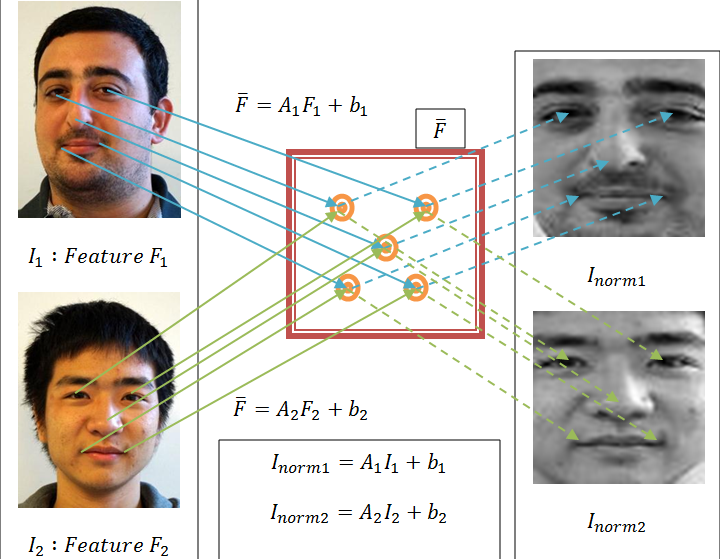
\includegraphics[width=0.7\linewidth]{./PCA1.png}
\caption{}
\end{figure}


In $ Figure 1 $, $ A_{i} $ and $ b_{i} $ are affine transformation matrix. Where $ A $ and $ b $ are given by:
$$
A = \begin{bmatrix} a_{11} & a_{12}\\ a_{21} & a_{22}\end{bmatrix} 
b = \begin{bmatrix} b_{1}\\ b_{2}\end{bmatrix} 
$$

\subsection*{How to compute A and b}

For each feature, the affine transformation is given by:
\begin{equation*}
f^{P}_{i} = Af_{i} + b
\end{equation*}
Where $ f_{i} $ is the feature location in original image and $ f^{P}_{i} $ is the position in normalization image. Since we already have $ f_{i} $ and $ f^{P}_{i} $ is also predetermined, let $ f = \begin{bmatrix} x\\ y\end{bmatrix} $, then the transformation can be written into:
\begin{equation*}
x^{P}_{i} = a_{11}x_{i} + a_{12}y_{i} + b_{1}
\end{equation*}
\begin{equation*}
y^{P}_{i} = a_{21}x_{i} + a_{22}y_{i} + b_{2}
\end{equation*}

We apply it on five features, the transformation is given by:
\begin{equation*}
 \begin{bmatrix} x1_{i} & y1_{i} & 1\\ x2_{i} & y2_{i} & 1\\ x3_{i} & y3_{i} & 1\\ x4_{i} & y4_{i} & 1\\ x5_{i} & y5_{i} & 1\end{bmatrix} 
 \begin{bmatrix} a_{11} & a_{21}\\ a_{12} & a_{22}\\ b_{1} & b_{2}\end{bmatrix} =  \begin{bmatrix} x1_{i}^{P} & y1_{i}^{P} \\ x2_{i}^{P} & y2_{i}^{P}\\ x3_{i}^{P} & y3_{i}^{P}\\ x4_{i}^{P} & y4_{i}^{P}\\ x5_{i}^{P} & y5_{i}^{P}\end{bmatrix} 
\end{equation*}
Until now, the problem convert to solve $ Ax=b $ in linear algebra. Since we got 10 equations for 6 unknowns, we employ SVD $( function \ pinv() \ in \ matlab )$ to solve it.

\subsection*{How to find $ \overline{F} $}
It is very important to get an appropriate $ \overline{F} $. We calculate $ \overline{F} $ by following steps:
\begin{itemize}
\item Step 1:
\item Step 2:
\item Step 3:
\item Step 4:
\item Step 5:
\end{itemize}

\section*{ $\llcorner$  Chapter 3: Principal Component Analysis $\urcorner$}
blablabla...

\section*{ $\llcorner$  Chapter 4: Recognition $\urcorner$}
blablabla...

\section*{ $\llcorner$  Chapter 5: Experimental Result and Analysis $\urcorner$}
blablabla...

\section*{ $\llcorner$  Chapter 6: Summary $\urcorner$}
blablabla...

\section*{ $\llcorner$  References $\urcorner$}

\end{document}
